\section{Síntesis y diagrama RTL detallado}

A continuación se presentan los diagramas RTL generados por Vivado a partir del código Verilog, que muestran la implementación estructural interna de los módulos principales del diseño.

\subsection{ALU}
En la Figura~\ref{fig:rtl_alu} se observa la implementación detallada de la Unidad Aritmético-Lógica. Cada operación aritmética/lógica se sintetiza en un bloque dedicado (ADD, SUB, AND, OR, XOR, corrimientos aritmético y lógico, INV). Sus salidas se combinan mediante un multiplexor (\texttt{RTL\_MUX}) gobernado por el código de operación \texttt{i\_op}.

\begin{figure}[H]
    \centering
    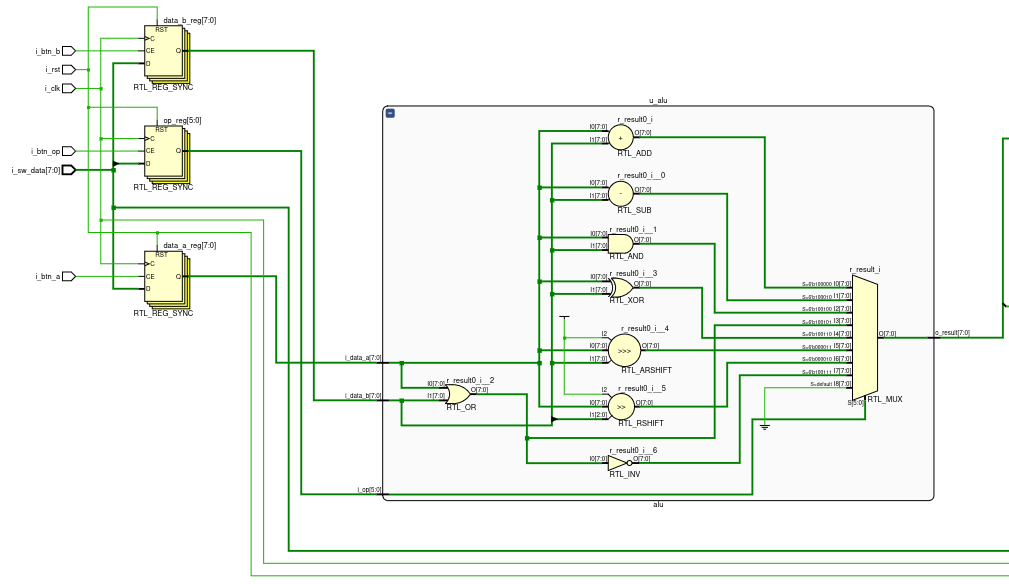
\includegraphics[width=\textwidth]{img/alu.png} % nombre de tu imagen
    \caption{Diagrama RTL del módulo \texttt{alu}.}
    \label{fig:rtl_alu}
\end{figure}

\subsection{Módulo de visualización (\texttt{sevenseg\_hex})}
La Figura~\ref{fig:rtl_disp} muestra el módulo de visualización. El bloque incluye:
\begin{itemize}
    \item Un divisor de frecuencia (\texttt{div\_reg}) que genera la señal de selección de dígito.
    \item Un multiplexor de nibbles (\texttt{RTL\_MUX}) para elegir cuál de los cuatro dígitos se presenta.
    \item Un decodificador hexadecimal a 7 segmentos (\texttt{RTL\_ROM}, \texttt{hex\_to\_sseg}).
    \item Un combinador (\texttt{RTL\_BMERGE}) para activar los ánodos (\texttt{o\_an}) de forma secuencial.
\end{itemize}

\begin{figure}[H]
    \centering
    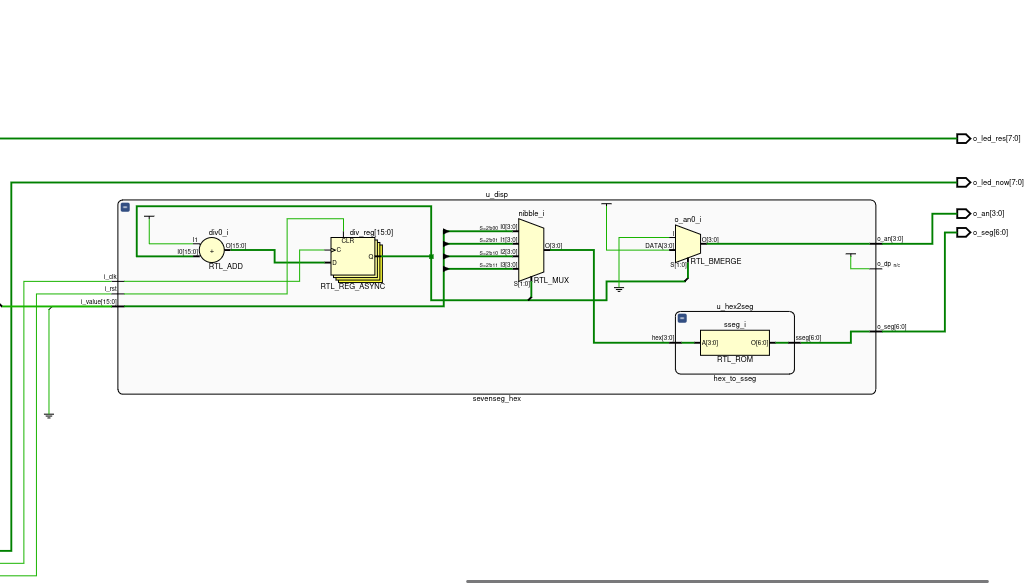
\includegraphics[width=\textwidth]{img/disp.png} % nombre de tu imagen
    \caption{Diagrama RTL del módulo de visualización \texttt{sevenseg\_hex}.}
    \label{fig:rtl_disp}
\end{figure}

\subsection{Módulo \texttt{top}}
Finalmente, en la Figura~\ref{fig:rtl_top} se muestra el diagrama RTL completo del bloque \texttt{top}, que integra los registros de entrada, la ALU y el módulo de display. Se observa cómo las señales de los botones y switches son capturadas en registros sincronizados, las operaciones se ejecutan en la ALU y el resultado se envía tanto a los LEDs (\texttt{o\_led\_res}) como al display de 7 segmentos.

\begin{figure}[H]
    \centering
    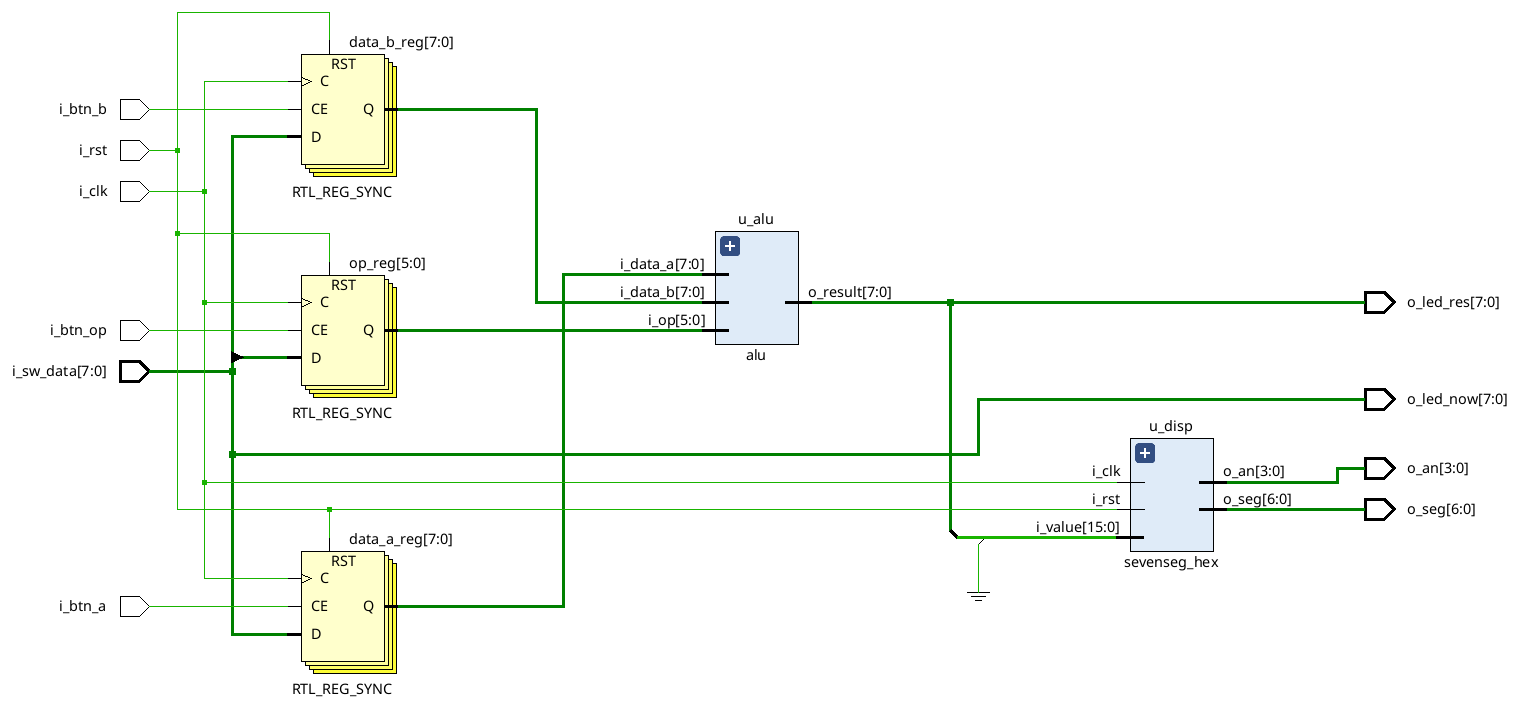
\includegraphics[width=\textwidth]{img/top.png} % nombre de tu imagen
    \caption{Diagrama RTL del bloque superior \texttt{top}.}
    \label{fig:rtl_top}
\end{figure}
